% Auteur : Steve Prud’Homme
% Cette oeuvre, création, site ou texte est sous licence Creative Commons Attribution - Pas d’Utilisation Commerciale - Partage dans les Mêmes Conditions 4.0 International. Pour accéder à une copie de cette licence, merci de vous rendre à l'adresse suivante 
% http://creativecommons.org/licenses/by-nc-sa/4.0/ ou envoyez un courrier à 
% Creative Commons, 444 Castro Street, Suite 900, Mountain View, California, 94041, USA.

% :::SNIPET
% ::: SECTION
% \section{Contexte} 
%		\begin{frame}[allowframebreaks]
%			\frametitle{}
%			\begin {itemize}
%				\item 
%			\end{itemize}
%		\end{frame}
%:::WATER MARK / FILIGRANE
%\usepackage{draftwatermark}
%\SetWatermarkLightness{0.5}
%\SetWatermarkAngle{25}
%\SetWatermarkScale{0.5}
%\SetWatermarkFontSize{2cm}
%\SetWatermarkText{Document de travail}


\documentclass{beamer}
\usepackage{color}
\usepackage{beamerthemesplit} % new 
\usepackage[french]{babel}
\usepackage[utf8]{inputenc}
\usepackage{tikz}
\usepackage[fixlanguage]{babelbib}
\selectbiblanguage{french}
% Natlib pour la bibliographie
\usepackage{natbib}
\usepackage{url}
\usetikzlibrary{mindmap,shadows,shapes,backgrounds}
\usepackage[T1]{fontenc}
\setbeamertemplate{bibliography item}[text]
\usepackage{multicol}


\definecolor{MightySlate}{RGB}{85,98,112}
\definecolor{Pacifica}{RGB}{78,205,196}
\definecolor{AppleChic}{RGB}{199,244,100}
\definecolor{CheeryPink}{RGB}{255,107,107}

\setbeamercolor{titlelike}{parent=structure}
\setbeamerfont*{title}{size=\huge}
\setbeamercolor{title}{bg=MightySlate, fg=white}
\setbeamercolor{author}{bg=Pacifica, fg=white}
\setbeamercolor{institute}{bg=AppleChic, fg=black}
\setbeamercolor{date}{bg=CheeryPink, fg=white}

\definecolor{DTUred}{RGB}{178,20,20}
\setbeamercolor*{palette primary}{use=structure,fg=white,bg=MightySlate}
\usepackage{helvet}
\usepackage{draftwatermark}
\SetWatermarkLightness{0.5}
\SetWatermarkAngle{25}
\SetWatermarkScale{0.5}
\SetWatermarkFontSize{2cm}
\SetWatermarkText{Document de travail}

\begin{document}
	\title{Survol des situations de travail, des processus de production, du contrôle de la qualité et des bonnes pratiques en conception et réalisation d’outils pédagogiques en ligne} 
	\author{Steve Prud'Homme} 
	\institute{GTN-Québec - Commission scolaire de Laval} 
	\date{\today} 

	
	%\usebackgroundtemplate{%
  %\includegraphics[width=\paperwidth,height=\paperheight]{sommaire.png}} 
	
	\frame{\titlepage} 
	\usebackgroundtemplate{ } 
	\section{Sommaire} 
		\begin{frame}
			Cette présentation vise à :
			\frametitle{Sommaire}
			\begin {itemize}
				\item 
			\end{itemize}
		\end{frame}
	\frame[allowframebreaks]{\frametitle{Ordre du jour}\tableofcontents}


	\section{Introduction} 
		\begin{frame}[allowframebreaks]
			\frametitle{}
			\begin {itemize}
				\item 
			\end{itemize}
		\end{frame}
		
	\subsection{Présentation} 
		\begin{frame}[allowframebreaks]
			\frametitle{Présentation}
			\begin {itemize}
				
                                \item 2010-2013 : enseignant au DEP em  infographie
                                \item 2013-2016 : Travail au sein d’une équipe de production d’outil pédagogique en ligne comme conseiller technopédagogique et comme intégrateur
                                \item 2013 : Pratique réflexive et de comparaison avec ce qui se fait déjà dans l’industrie d’arts graphiques
                                \item 2013 : Membre du GTN-Québec
                                \item 2014-2015 : Survol des situations de travail, des processus de production, du contrôle de la qualité et des bonnes pratiques en conception et réalisation d’un outil pédagogique en ligneProjet de   
			\end{itemize}
		\end{frame}
			
            \subsection{Objectifs de la présentation} 
		\begin{frame}[allowframebreaks]
			\frametitle{Objectifs de la présentation}
			\begin {itemize}
				
                                \item La problématique
                                \item Cadre de référence
                                \item Méthodologie
                                \item Résultats
                                \item Suite ou interprétation
                        \end{itemize}
		\end{frame}

               \section{Problématique} 
		\begin{frame}[allowframebreaks]
			\frametitle{}
			\begin{itemize}
				\item 
			\end{itemize}
		\end{frame}

               \subsection{Contexte d'émergence} 
		\begin{frame}[allowframebreaks]
			\frametitle{Contexte d'émergence}
			\begin{itemize}
				\item Production de l'AEP en service de garde en ligne version 1
                                  \begin{itemize}
                                    \item L’équipe multidisciplinaire de production a vécu son lot de difficultés
                                    \item L’équipe de travail a été confrontée à un écart considérable entre le travail visé et la réalité de production.
                                    \item Cette réalité a amené l’équipe à porter une réflexion sur les pratiques dans le but de mieux comprendre ce qui ne fonctionnait pas dans son processus de production.
                                  \end{itemize}
                                \framebreak
                                \item Le défi de la version 2 de l'AEP service de garde en ligne
                                  \begin{itemize}
                                  \item Guider l’équipe de travail et les membres de la direction vers de nouvelles pratiques
                                  \item Faire preuve de tact avec l’équipe de travail et les membres de la direction afin de les amener à une réflexion sur leurs pratiques. 
                                  \item Production d'un premier document intitulé : « Projet de flux de production d’un projet de cours en ligne » 
                                    \begin{itemize}
                                      \item Ce document traite des balises et limites d’un tel flux de production pour un projet de cours en ligne et ses constituantes
                                      \item Ce flux de production inclut inclut les tâches, les livrables et les points de contrôles, tout en définissant les principaux concepts liés, les matériaux d’un projet de cours en ligne.
                                         
                                    \end{itemize} 
                                  \end{itemize}                                             
                                \end{itemize} 
                        \end{frame}

  \subsection{Contexte d'application} 
		\begin{frame}[allowframebreaks]
			\frametitle{Contexte d'application}
			Plusieurs écrits documentent la conception d’outil pédagogique en ligne, mais le point de vue des auteures ou des auteurs diverge sur les différentes étapes nécessaires à leur réalisation \citep[p.18]{bonneau2013a}.
                   \begin{figure}
                     \centering
                     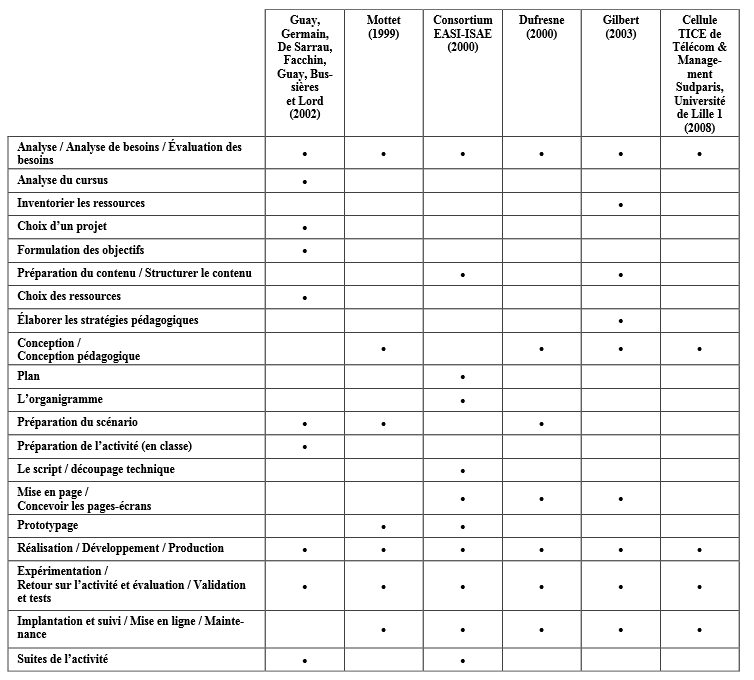
\includegraphics[width = 0.52\textwidth]{tableau6methodes.png}
                     \caption{\tiny{Tableau comparatif des étapes de six méthodes utilisées pour la conception et la réalisation d’outils pédagogiques en ligne \citep[p.20]{bonneau2013a}}}
                   \end{figure}
                   \begin{itemize}                   
                   \item On constate donc qu’il y a une grande disparité entre les méthodes et que, comme le dit \citet{bonneau2013a} , peu font l’unanimité. 
                   \item La variété des méthodes pourrait s’expliquer par le fait que les outils pédagogiques en ligne sont protéiformes, c’est-à-dire qui peut prendre diverses formes.
                   \item Il faut donc demeurer critiques sur l’application d’un processus systématique
                   \item \citet[p.10]{retalis1997a}, \citet[p.46]{smith2006a} et \citet[p.3]{pohl2004a} le confirment.
                   \end{itemize}
			\par \citet[p.3]{pohl2004a} prétend que : 
			\par« Guidelines for the development of e-learning systems have advantages and disadvantages. One disadvantage is that it is sometimes difficult to generalize guidelines. Related to that is the fact that the efficiency of educational media always depends on the context in which they are used. Guidelines should, therefore, not be formulated as cookbook recipes but rather be flexible tools which can be adapted to various different situations and environments. If such a flexible approach is used, guidelines can be applied quite effectively ».
			\par  Il a donc fallu prévoir, lors du survol, traiter de l’aspect de la situation de travail: soit du contexte dans le cadre duquel les processus sont utilisés.
                \end{frame}

\subsection{Milieu et les personnes concernées} 
		\begin{frame}[allowframebreaks]
			\frametitle{Précision sur le milieu et les personnes concernées}
                        \
                        \begin{itemize} 
                        \item  Les équipes sont multidisciplinaires ;
                        \item Composées de spécialistes des contenus qui peuvent être des enseignants, des spécialistes de la formation ou des conseillers pédagogiques ;
                        \item Ces équipes sont formées de : 
                        	\begin{itemize}
                        		\item concepteur pédagogique / conseillers pédagogiques ou technopédagogiques,
                        		\item intégrateurs, les infographistes, les programmeurs, les spécialistes des réseaux,
                        		\item de chargés de projets ou gestionnaires dirigent les projets.
                        	\end{itemize}

                        \end{itemize}

             
                \end{frame}

\subsection{La nécessité} 
		\begin{frame}[allowframebreaks]
			\frametitle{La nécessité d’un survol}
                        
                        \begin{itemize} 
                        \item  Les méthodes dans le domaine de la conception et de la réalisation d’outils pédagogiques en ligne sont importantes \citep[p. 842]{bohl2002a}, \citep[p. 218]{barry2003a}, \citep[p. 1]{hadjerrouit2007a} tirés de \cite{bonneau2013a};
                        \item La conception et la réalisation d’outils pédagogiques en ligne sont souvent faites par des novices en la matière \citep[p. 351]{verstegen2008a} tiré de \citet{bonneau2013a};
                        \item Les enseignants semblent avoir une vision restreinte au niveau de l’ampleur et de la complexité (voire l’entièreté des problèmes) que l’appropriation d’une telle pratique peut créer, soit une vision générale de tout le processus engendré par une telle démarche dans un dispositif de FAD \citep[p. 105]{roy2011a} tiré de \citet{bonneau2013a}; 
                        \item Les méthodes d’ingénierie pédagogique comme la méthode ADDIE,aurais provoqué une simplification de la perception qu’ont de nombreux acteurs du domaine de l’éducation de ce processus\citep[p.28]{bonneau2013a}. 
                        \item En récupérant une méthode d’ingénierie pédagogique pour en faire une méthode de conception et de réalisation d’outil pédagogique en ligne, on propage l’idée que ce processus est simple, pour ne pas dire simpliste\citep[p.29]{bonneau2013a}.
                        \item Il y aurait peut-être necessité d'une d’une méthode synthèse issue des travaux de recherche et de ce qui se fait dans la réalité.

                        \end{itemize}

             
                \end{frame}
                
                \subsection{Objectif général} 
		\begin{frame}
			\frametitle{Objectif général}
                        
                        \begin{itemize} 
                        \item  Quelles sont les situations de travail, les processus de production, du contrôle de la qualité et de bonnes pratiques en conception et réalisation d’outil pédagogique en ligne dans le milieu des producteurs d’outil pédagogique en ligne québécois et ce pour la plupart des milieux soit la FGJ, FGA, FP, le CÉGEP, l’université et l’entreprise privée? 
                         \item Quelles sont les voies à privilégier afin d’améliorer les failles notées et rendre ce travail plus efficient?

                        \end{itemize}

             
                \end{frame}
                
	\section{Méthodologie} 
		
                        
				\subsection{Type de recherche} 
					\begin{frame}
						\frametitle{Type de recherche}
                        
                        			\begin{itemize} 
                       				 \item Étude de 6 cas de producteurs d’outil pédagogique en ligne. 
                       				 \item Travail d’analyse par théorisation ancrée 
                       				 \item Codification, catégorisation et mise en relation 

                       		 \end{itemize}
				\end{frame}
                       	\subsection{Déroulement de la recherche} 
					\begin{frame}[allowframebreaks]
						\frametitle{Déroulement de la recherche}
                        
                        			\begin{itemize} 
                       				 \item Recensement normes et standards de qualité en e-learning
                       				 \item Entretiens avec des producteurs d’outil pédagogique en ligne font partie de l’échantillon. 
                       				 \item Les notes, traces documentaires et verbatim de ces entretiens servent de matières premières à la recherche 
                       				 \item Analyse en profondeur :
                       				 \begin{itemize} 
                       				 	\item des situations de travail, 
                       				 	\item des processus de production
                       				 	\item du contrôle de la qualité
                       				 	\item des bonnes pratiques et 
                       				 \end{itemize}
                       				 \item Élaboration de la typologie qui permet de :
                       				 \begin{itemize} 
                       				 	\item nommer,
                       				 	\item regrouper 
                       				 	\item hiérarchiser les différentes étapes des méthodes étudiées,
                       				 	\item validation de la typologie par des experts, 
                       				 	\item élaboration des matrices de comparaison.
							\end{itemize}
                       		 \end{itemize}

             
                \end{frame}
                     	\subsection{Population à l’étude} 
					\begin{frame}[allowframebreaks]
						\frametitle{Population à l’étude}
                        
                        			\begin{itemize} 
                       				 \item Recensement normes et standards de qualité en e-learning
                       		              \item La population cible est constituée de 6 producteurs d’outil pédagogique en ligne. 										 \item L’échantillon est le plus grand possible dans les limites et les contraintes financières. 
                       		              \item L’ensemble des interviews ont produit : 
                       		              \begin{itemize} 
                       		              	\item 10 heures d’entretien
                       		              	\item plus de 350 pages de verbatim
                       		              	\item plus de 20 documents trace.
                       		              \end{itemize}
                       		 \end{itemize}
                       		 \end{frame}
				\subsection{Critères de sélection} 
					\begin{frame}[allowframebreaks]
						\frametitle{Critères de sélection}
                        
                        			\begin{itemize} 
                       				\item Être disponibles.
							\item Provenir :
							\begin{itemize}
								\item de l’entreprise, 
								\item de la formation générale des jeunes, de la formation générale des adultes ou de la formation professionnelle, 
								\item du CÉGEP, 
								\item de l’université 
								\item de l’entreprise privée.
							\end{itemize}
							\item Avoir des petites organisations proches des enseignants comme des grandes organisations ayant de grosses équipes de production
                       		 \end{itemize}
                       		 \end{frame}
                       		 \subsection{Échantillon} 
					\begin{frame}[allowframebreaks]
						\frametitle{Échantillon}
                        
                        			\begin{itemize} 
                       				\item Producteur 1 : un CÉGEP produisant des outils pédagogiques en francisation encadrés par le Ministère de l’Immigration de la Diversité et de l'Inclusion.
                       				\item Producteur 2 : une microentreprise produisant des outils pédagogiques pour les entreprises et expertes dans l’accompagnement des organismes dans les étapes de préproduction.
							\item Producteur 3 : un partenariat public privé producteur d’outils pédagogiques en ligne pour la formation générale des jeunes et la formation générale des adultes.
							\item Producteur 4 : une PME produisant des outils pédagogiques en ligne pour des entreprises et des organismes publics.
							\item Producteur 5 : un centre de formation professionnelle producteur d’outils pédagogiques pour une attestation de spécialisation professionnelles (ASP) encadré par le MEESR.
							\item Producteur 6 : une grande université produisant des outils pédagogiques en ligne pour plusieurs programmes d’études ou cours en ligne.

                       		 \end{itemize}
                       		           
                \end{frame}
                       		 
                       		 \subsection{Les techniques et instruments de collecte de données} 
					\begin{frame}[allowframebreaks]
						\frametitle{Les techniques et instruments de collecte de données}
                        
                        			\begin{itemize} 
                       				\item L’approche semi-dirigée a d’abord été utilisée afin de mieux comprendre :
                       				\begin{itemize}
                       				 	\item les processus de production, 
                       				 	\item le contrôle de la qualité 
                       				 	\item les bonnes pratiques 
                       				 \end{itemize}
                       				\item L’approche dirigée a été utilisée afin de mieux comprendre :
                       				\begin{itemize}
                       					\item les situations de travail 
                       					\item les demandes et les attentes
                       					\item écarts entre la tâche telle que prévue et l’activité réelle de travail
                       					\item bilan des difficultés rencontrées conséquences possibles du travail 
							\end{itemize}
							\item Une grille préliminaire d’analyse lors des entretiens
							\item Analyse des traces (des documents pertinents à la compréhension)
							\item Des enregistrements sonores ont été produits lors des entretiens
							\item Les enregistrements sonores ont été transcrits sous forme de verbatim qui ont été analysés à l’aide du logiciel nVivo
                       		 	\end{itemize}
                       		           
                			\end{frame}
                
                  \section{Résultats} 
                  \subsection{Normes de qualité} 
					\begin{frame}[allowframebreaks]
						\frametitle{Recension des normes de qualité en production d’outils pédagogiques en ligne}
                        La recherche documentaire, démontre qu’il existait 3 grandes catégories de normes. 
                        			\begin{itemize} 
                       				\item Outils de contrôle de la qualité de l’éducation,
                       				\item Normes technologiques en e-learning. 
                       				\item Normes de qualité dédiées à l’e-learning.
                       		 	\end{itemize}
                       		 \end{frame}                   
                  \subsection{Outils de contrôle de la qualité de l’éducation} 
					\begin{frame}[allowframebreaks]
						\frametitle{Outils de contrôle de la qualité de l’éducation}
                        			\begin{description}[Second Item]
							
							\item[Chartes] est un outil déontologique.
							\begin{itemize}
								\item Elle ne comporte pas de critère mesurable
								\item Elle énonce des engagements du fournisseur envers ses clients.
							\end{itemize}
							
							\framebreak
							
							\item[Labels] engagent une tierce partie dans la relation qui unit le client à son fournisseur. 
							\begin{itemize}
								\item Ils sont accordés par un organisme extérieur à l’organisme de formationl. 
								\item Ne concernent pas le contenu des formations. 
								\item Une démarche commerciale 
								\item Exemple, au Canada, : Red Flag ou le CPMT
							\end{itemize}
							
							\framebreak
							
							\item[Certifications] de tierces parties accréditées, il y en a deux types :
							\begin{itemize}
								\item certifications de services : 
								\begin{itemize}
									\item nécessité d’un éclaircissement dans le domaine des services, en l’absence de sigle officiel en guise de qualité,
									\item exemple 1 : les différents cadres de référence produits par le MEESR servent de certification de service au Québec, 
									\item exemple 2 :  en France, un organisme indépendant produit ces certifications de services, il s’agit de l’AFNOR ;
								\end{itemize}
								
								\framebreak
								
								\item standards d'assurance qualité :
								\begin{itemize}
								\item posent des principes de management,
								\item  s’appliquent à tous les secteurs d’activité de façon non spécifique,
								\item décrivent une organisation interne, propre à chaque organisation,
								\item visent à minimiser les risques de dysfonctionnement grâce à l’application de procédures,
								\item contrat transparent avec le client ou l’a, qui peut être l’apprenant
								\item exemple 1: En mai 2000, 250 organismes ayant pour activité principale la formation professionnelle avaient été certifiés par la norme ISO 9001-1994 en France.
								\item exemple 2 :  Au Québec, les normes de qualité ISO sont peu adoptées en éducation et en formation continue, même sur le plan des entreprises. Selon le BNQ , 2 organismes publics étaient certifiés ISO9001 en 2015 , et 1 entreprise de formation.
								\end{itemize}
								   
							\end{itemize}
						
						\framebreak
						
						\item[Technologiques] Il existe une grande variété de standards techniques :  
							\begin{itemize}
							\item beaucoup sont de l’ordre de la structuration et de la description des métadonnées, 
							\item d’autres sont pour les paquetages de cours (SCORM, AICC, etc.),
							\item il s’agit de spécifications techniques, 
							\item bien qu’elles soient utilisées par nos producteurs, il ne s’agit pas, dans le cadre de ce travail, de notre principal champ d’intérêt ;
							\end{itemize}
						
						\framebreak
						
						\item[Dédiés] Parmi les normes de l'e-learning, nous comptons :
							\begin{itemize}
							
							\framebreak
							
							\item QUALITÉ TOTALE  
								\begin{itemize}
								\item s’intéresse davantage à l’organisme d’e-learning que directement à ses clients
								\item elle permet de promouvoir la gestion de la qualité au sein des organismes d’e-learning
								\item elle permet de rechercher les bonnes pratiques dans une démarche d’auto-évaluation. 									
								\framebreak
								
								\item exemple : la SOFEDUC a écrit 10 normes qui s’intéressent :
								 	\begin{itemize} 
								 	\item au besoin de formation
								 	\item aux objectifs d’apprentissage,
								 	\item aux formateurs,
								 	\item aux contenus des formations,
								 	\item aux stratégies de formation,
								 	\item à l’évaluation des apprentissages,
								 	\item à l’évaluation de l’activité ou du programme de formation,
								 	\item à l’unité responsable
								 	\item au système d’amélioration continue,
								 	\item aux dossiers des participants ;
								 	\end{itemize}
								 \end{itemize}
							
							\framebreak
							
							\item QUALITY STANDARDS FOR EVALUATING MULTIMEDIA AND ONLINE TRAINING  
								\begin{itemize}
								\item permet d’estimer comment un cours en ligne satisfait aux exigences fondamentales de la qualité dans chacun des quatre champs suivants : 
									\begin{itemize}
									\item les besoins organisationnels,
									\item le contenu pédagogique,
									\item la convivialité
									\item l’architecture des instructions pour l’enseignement. 
									\end{itemize}
								\end{itemize}
							
							\framebreak
							
							\item QUALITY IN OPEN AND DISTANCE LEARNING, QUALITY CONCIL (ODL/QC) 
								\begin{itemize}
								\item complémentaire aux précédentes et s’intéresse à : 
									\begin{itemize}
									\item l’inscription et à l’accompagnement des élèves
									\item l’environnement d’apprentissage
									\item l’offre du fournisseur de ressources
									\item aux clauses du contrat de formation. 
									\end{itemize}
								\item Il s’agit d’une accréditation qui peut être obtenue sur présentation d’un dossier et après
								 une visite.	
								\end{itemize}
							
							\framebreak
							
							\item DISTANCE LEARNING GUIDELINES 
								\begin{itemize}
								\item composée d’un ensemble de documents qui définissent les normes de qualité pour la conception du programme : 
									\begin{itemize}
									\item la prestation, 
									\item l’accompagnement des apprenants, 
									\item les modalités de communication avec l’apprenant,
									\item l’évaluation de l’apprenant, 
									\item le travail de groupe.
									\end{itemize}
								\end{itemize}
							
							\framebreak
							
							\item Autres normes
								\begin{itemize}
								\item ISTE : sert à préparer l’enseignant et l’apprenant au meilleur usage des technologies dans la nouvelle société de l’information
								\item DITRA : est un programme de la communauté européenne plus particulièrement dédié à la construction de modèles de compétences requises par les acteurs de l’e-learning, dans les diverses étapes de sa conception et de son utilisation
								\item GUIDE DES BONNES PRATIQUES POUR DÉVELOPPER LES COMPÉTENCES PAR LE NUMÉRIQUE DU CÉFRIO : qui est un survol des usages et bonnes pratiques pour les projets de formation avec le support des TIC. 
								\item LABEL OPQF : est quant à lui attribué en reconnaissance du professionnalisme d’un produit, de ses compétences, et de l’expérience professionnelle dans un ou plusieurs domaines de qualification sélectionnés parmi les 19 domaines existants.
								\end{itemize}
							\end{itemize}						
						\end{description}
		 \end{frame}   
		 
		 \subsection{Acteurs} 
					\begin{frame}[allowframebreaks]
						\frametitle{Acteurs}
                        			Nous avons tenté, pour chaque participant, de cerner les personnes ou organismes qui sont appelées à contribuer à la production d’un outil pédagogique en ligne.
							\begin{itemize}
							\item Grandes variétés d'acteurs
							\item Les acteurs sont de l'interne et de l'externe
							\item Multidisciplainaire
								\begin{itemize}
								\item Acteurs recherche
									\begin{itemize}
									\item CNT (conseiller en nouvelles technologies
									\item Conseillère en recherche et développement (CRD)
									\end{itemize}
								\item Acteurs techniques													
								\item Acteurs pédagogiques
									\begin{itemize}
									\item Contenu
									\item Conception pédagogique
									\item Conception technopédagogique
									\item Droits d'auteur
									\item Environnement numérique d'apprentissage
									\end{itemize}
								\item Client
									\begin{itemize}
									\item Apprenant
									\item Entreprises
									\item OSBL
									\item Organismes publics comme clients (ministères, commissions scolaires, écoles et centres)
								\end{itemize}
								\item Acteurs créatifs
									\begin{itemize}
									\item Spécialistes Web
									\item Image
									\item Vidéo
									\item Multimédia
									\item Audio
									\end{itemize}
								\item Grands acteurs du Web		
									\begin{itemize}
									\item Grands services infonuagiques tels que Google
									\item Réseaux sociaux
									\end{itemize}
								\item Acteurs du contrôle de la qualité
									\begin{itemize}
									\item Réviseurs
									\item Testeurs 
									\item Responsable de la qualité
									\end{itemize}
								\item Acteurs en gestion
								\end{itemize}
							\item La démocratisation des outils diminue le nombre d'acteurs
							\item La complexité des outils augmentent le nombre d'acteurs spécialisés
							\end{itemize}
						
					\end{frame}
					
					
					
					 \subsection{Étapes de production} 
						\begin{frame}[allowframebreaks]
						\frametitle{Étapes de production}
                        			Nous avons tenté, pour chaque participant, de cerner l’ensemble des phases nécessaires à la transformation des matières premières en produits finis.
						\begin{itemize}
						\item Grandes variétés d'étapes
						\item Les organisation moins spécialisées ont un processus de production moins développé
						\item Les organisation moins spécialisées n'ont pas de processus l'analyse préliminaire
						\item Peu d'organisation utilisent des méthodes de gestion de projet itérative ou organique
						\item Les organisations spécialisées sont fortement influencé par l'ADDIE.
						\end{itemize}
						Voici les principales étapes de production observées :	
						\begin{itemize}
						\framebreak
						\item Avant le projet
							\begin{itemize}
							\item Analyse préliminaire, pré-projet, avant-projet, analyse du besoin ou d'une problématique, première discussion, tempête d’idées
							\item Test des dispositifs de la competition.
							\item Analyse du contenu : modélisation de connaissances, inventaire de que le client détient déjà (contenu et matériel), définition des apprentissages doivent être produits,organisation du contenu d’apprentissage :
							\item Conception
								\begin{itemize}
								\item Production de documents papier et  correction sur le matériel écrit
								\item Prototypage, esquisses, confrontation, ébauche, micro et macrodesign
								\end{itemize}
							\end{itemize}
						\framebreak
						\item Pendant le projet
							\begin{itemize}
							\item Production
							\item Développement
								\begin{itemize}
								\item Médiatisation
								\item Production des composantes
								\item Assemblage sur un environnement numérique d'apprentissage
								\item Tests
								\item Il est possible pendant la phase de productio qu'on travailler sur la deuxième version d'un projet
								\end{itemize}
							\item Implantation
								\begin{itemize}
								\item Prétest
								\item Prestation,
								\item Évaluation des étudiants et du cours
								\item Post-prestation
								\item Archivage
								\end{itemize}
							\end{itemize}
						\framebreak
						\item Après le projet
							\begin{itemize}
							\item Bilan et analyse de la prestation.
							\item Évaluation
								\begin{itemize}
								\item évaluation technique
								\item test par des humains (enseignants, élèves, etc.)
								\item correction pour faire suite aux tests effectués par les élèves
								\end{itemize}
							\end{itemize}	
						\item Processus d'amélioration continue (peu mentionné)
								\begin{itemize}
								\item Amélioration de session en session.
								\item Rencontre hebdomadaire ou bihebdomadaire en comité
								\end{itemize}
						\end{itemize}		
							
						
					\end{frame}
							
						
						 \subsection{Livrables} 
						\begin{frame}[allowframebreaks]
						\frametitle{Livrables}
                        			Nous avons tenté, pour chaque participant, de cerner l’ensemblre des résultats attendus dans le cadre d’un projet d’outils pédagogique en ligne et qui seront matérialisés par un produit, un document de référence ou une activité.
						\begin{itemize}
							\item Grandes variété de livrables
							\item Les organisations moins spécialisées focussent sur les outils pédagogiques en lignes finaux
							\item Les organisations plus spécilisées mettent plus d'emphase sur les livrables de planification comme l'analyse préliminaire ou l'analyse du contenu.
							\item Les organisations moins spécliasées substituent ce qui est fait dans la classe
						\end{itemize}		
						Nous avons observés 7 types de livrables
						\begin{itemize}
							\item Les livrables en lien avec la planifications
							
							\item Les livrables en lien avec la conception
							\item Les livrables en lien avec la production
							\item Les livrables en lien avec le prototypage
							\item Les livrables en lien avec le produite finale
							\item Les livrables en lien avec le contrôle de qualité
							\item Les livrables en lien avec l'implantation
							\item Les livrables en lien avec les données
						\end{itemize}
						
					\end{frame}


\section{Bibliographie}
\subsection{Bibliographie}
\frame[allowframebreaks]{\frametitle{Bibliographie}

\bibliographystyle{apalike}
\bibliography{bibliographie} %bibtex file name without .bib extension
}
\end{document}

